\subsection{Performance Evaluation}
\label{sec:evaluation}
%We have compared the processing time of each user login in UPRESSO, with the original OIDC implementation (MITREid Connect) and SPRESSO which only hides the user's accessed RPs from IdP.
%OIDC, RP的软件
\noindent\textbf{Environment.} The evaluation was performed on 3 machines, one (3.4GHz CPU, 8GB RAM, 500GB SSD, Windows 10) as IdP, one (3.1 GHz CPU, 8GB RAM, 128 GB SSD, Windows 10) as an RP, and the last one (2.9GHz CPU, 8GB RAM, 128GB SSD, Windows 10) as a user. The user agent is Chrome v75.0.3770.100. And the machines are connected by an isolated 1Gbps network.

%RP(不包括特定方案的SDK)大约需要230行JAVA代码
%OIDC(MITREid)的SDK需要大约20行的JAVA代码,需要额外添加一个HTML文件(包含大约20行JavaScript代码)
%UPRESSO的SDK需要大约1100行代码,不需要添加额外的HTML文件
%OIDC和UPRESSO的SDK只需要RP提供两个网络接口(网址),然后在对应的网络接口中引用对应的API(每个接口对应一个API,分别命名为tokenRequestGenerate和userAccountAchieve),其他的处理流程均由SDK完成
%SPRESSO由于结构与OIDC完全不同,所以使用了SPRESSO提供的RP的开源代码
For better evaluation, we build one RP for both UPRESSO and MITREid Connect which is also implemented  based on Spring Boot framework, as well as the identity proof transmission from user to RP in MITREid Connect is implemented by JavaScript running in RP's web page. The IdP in MITREid Connect is achieved from github~\cite{MITREid}. However, the SPRESSO system is downloaded from~\cite{spressome} containing IdP, RP and FWD. 

%A DELL OptiPlex 9020 PC (Intel Core i7-4770 CPU, 3.4GHz, 500GB SSD and 8GB RAM) with Window 10 prox64 works as the IdP. A ThinkCentre M9350z-D109 PC (Intel Core i7-4770s CPU, 3.1GHz, 128GB SSD and 8GB RAM) with  Window 10 prox64 servers as RP. The user adopts Chrome v75.0.3770.100 as the user agent on the Acer VN7-591G-51SS Laptop (Intel Core i5-4210H CPU, 2.9GHz, 128GB SSD and 8GB RAM) with  Windows 10 prox64. For SPRESSO, the extra trusted entity FWD is deployed on the same machine as IdP.
%没有因为部署在同一个机器上使得开销变长,monitor指系统的监视器
%The monitor demonstrates that the calculation and network processing of the IdP does not become a bottleneck (the load of CPU and network is in the moderate level).

\noindent\textbf{Setting.} We have measured the time for a user's login at an RP, and calculated the average values of $1000$ measurements.
For better analysis, we divide a login into 4 phases according to the lifecycle of identity proof: \textbf{Identity proof requesting} (Steps 1-2.5 in Figure~\ref{fig:process}), RP (and user) constructing and transmitting the request to IdP; \textbf{Identity proof generation} (Step 4 in Figure~\ref{fig:process}), IdP generating identity proof (no user authentication); \textbf{Identity proof transmission} (Steps 5.1-5.3 in Figure~\ref{fig:process}), IdP (and user) transmitting the identity proof to RP server; and \textbf{Identity proof verification} (Steps 6 in Figure~\ref{fig:process}), RP verifying and parsing the identity proof.

\noindent\textbf{Results.}
The evaluation results are provided in Figure~\ref{fig:evaluation}. The overall processing times are  113 ms, 308 ms and 208 ms for MITREid Connect, SPRESSO and UPRESSO, respectively. The details are as follows.

\begin{figure}
  \centering
  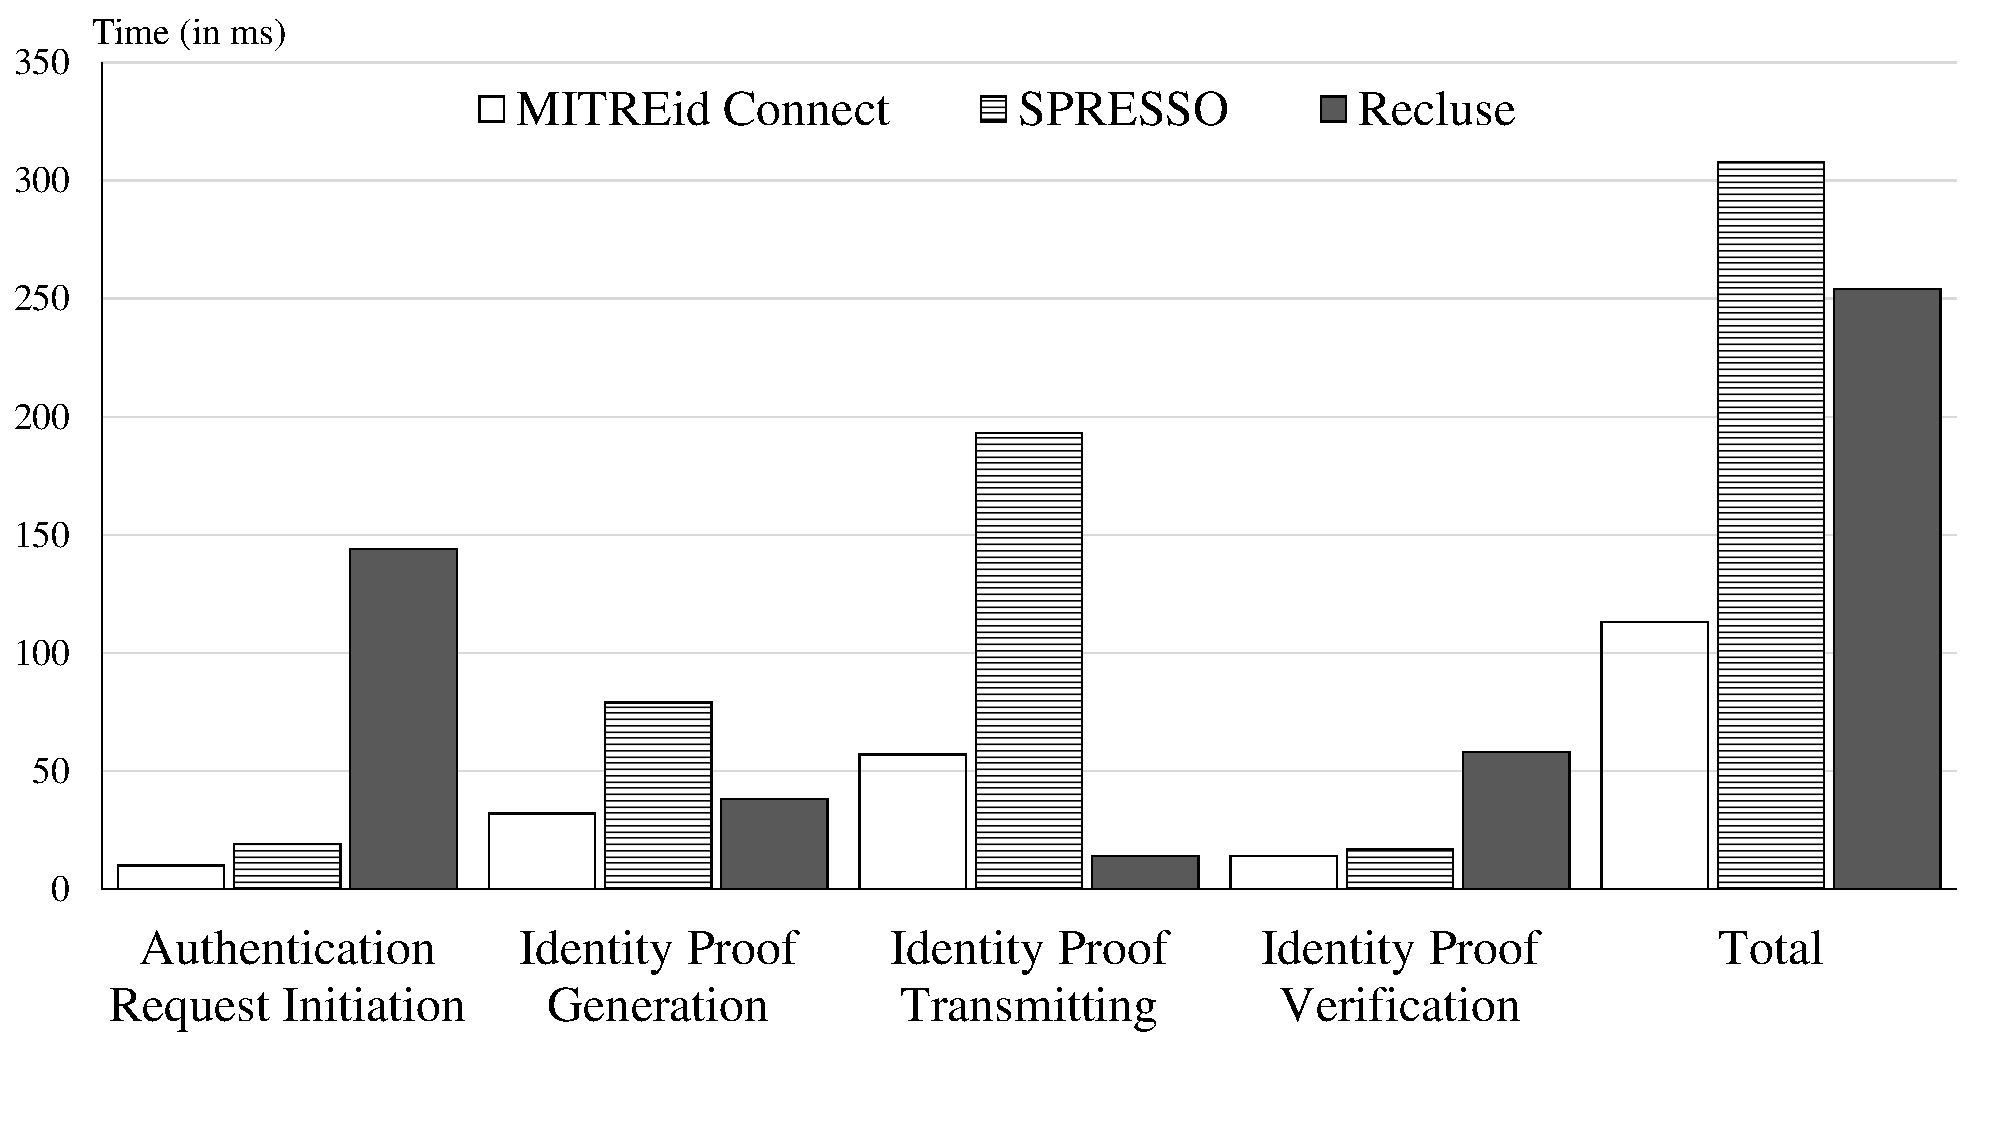
\includegraphics[width=\linewidth]{fig/evaluation2.pdf}
  \caption{The Evaluation.}
  \label{fig:evaluation}
\end{figure}

In the requesting, UPRESSO requires the user and RP to perform 1 and 2  modular exponentiations respectively for $PID_{RP}$ transforming and cooperatively complete $PID_{RP}$ refreshing at the IdP, which totally needs 98 ms;  SPRESSO needs 19 ms for the RP to obtain IdP's public key and encrypt its domain; while MITREid Connect only needs 10 ms.

%估计能减少多少,
In the generation, UPRESSO needs  an extra 6 ms for computing $PID_U$, compared to MITREid Connect which only needs 32 ms.
SPRESSO requires the longest time (71 ms), as it adopts a JavaScript cryptographic library, while others adopt a more efficient Java library.

%transmission & extraction
In the transmission, UPRESSO only needs 14 ms for Chrome extension to relay the identity proof to RP server directly.
MITREid Connect requires the IdP to send the identity proof to  RP's web page which then sends the proof to RP server through a JavaScript function, and needs 57 ms.
SPRESSO needs the longest time (193 ms) due to a complicated processing at the user's browser,
  which needs the browser to obtain identity proof from IdP, download the JavaScript program from a trusted entity (named FWD), execute the program to decrypt RP's endpoint, send this endpoint to RP's web page who finally transmits the proof to RP server.
In the evaluation,  FWD and IdP are deployed in one machine, which doesn't introduce performance degradation as  FWD and IdP work sequently for one login.

%SPRESSO needs a trusted entity named FWD for transmitting the identity proof. We deployed FWD and IdP on the same machine to reduce transmitting delay between them, while the computation never becomes the bottleneck according to the observation.


In the verification, UPRESSO needs an extra calculation for $Account$, which then requires  58 ms, compared to 14 ms in MITREid Connect and 17 ms in SPRESSO.



